\chapter{Directional Noise Elimination}\label{ch:directional}
This chapter deals with directional filtering. In the beginning, the prerequisites for 
the filtering idea are presented. Afterwards, the actual filtering idea is shown and explained.
In the end, the results are presented, and a conclusion is drawn.
\section{Concept}
Figure \ref{fig:2sources} shows a scenario where directional filtering could be used.
Source 1 and Source 2 are both talking simultaneously. At the origin, two microphones,
left (L) and right (R) are fixed and recording.

\begin{figure}[htp]
	\centering
	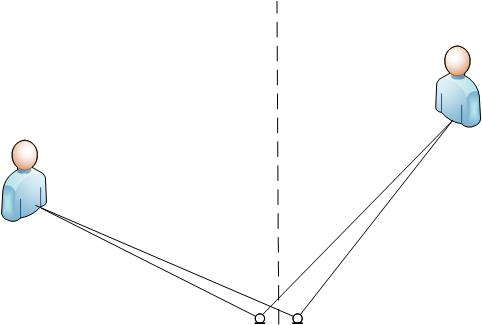
\includegraphics[width=0.65\textwidth]{Illustrations/2sources.jpg}
	\caption{Two Persons Talking}
	\label{fig:2sources}
\end{figure}

Due to the nature of the setup, the microphones will record  both the speakers.
However, both microphones record two persons talking. As a consequence, each microphone
returns a soundwave containing two signals. The aim is to filter out one of them
by only using the two soundwaves available.

In order to be able to do this, one assumption needs to be made. That is, that the 
angle at which each source is located, is known.

\begin{figure}[htp]
	\centering
	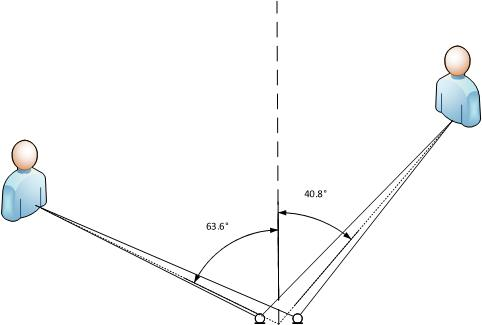
\includegraphics[width=0.67\textwidth]{Illustrations/2sourcesWangles.jpg}
	\caption{Two Persons Talking With Known Angles}
	\label{fig:2sourcesWangles}
\end{figure}

Figure \ref{fig:2sourcesWangles} represents the same scenario. However this time, the angles
of the sound sources are known. The Sources and the Origin are represented with coordinates.
This helps in determining the formulas that are needed in order to obtain the delay in samples.

\begin{figure}[htp]
	\centering
	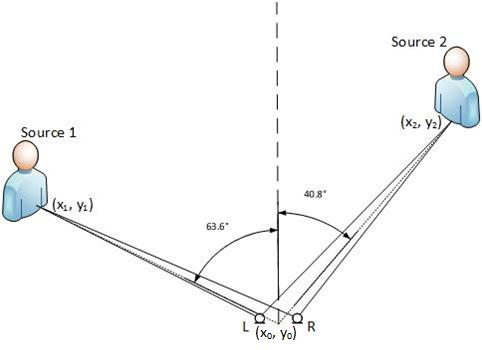
\includegraphics[width=0.67\textwidth]{Illustrations/2sourcesWanglesAndPossition.jpg}
	\caption{Two Persons Talking With Known Angles}
	\label{fig:2sourcesWanglesAndPossition}
\end{figure}

\newpage

Figure \ref{fig:zoomedin1} represents the delay between the two signals. One advantage
is represented by the fact that, no matter the distance of the source, the delay between the
signals is always the same. By knowing the angle, the sampling frequnecy and the travelling
speed of sound, the delay in samples can be determined.


\begin{figure}[htp]
	\centering
	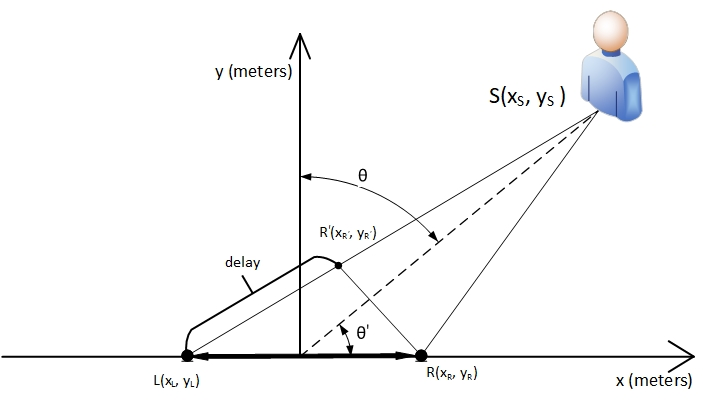
\includegraphics[width=0.65\textwidth]{Illustrations/delayDrawingForEquations.jpg}
	\caption{Delay}
	\label{fig:zoomedin1}
\end{figure}

\newpage
\section{Mathematical Solution}

Figure \ref{fig:zoomedin2} is a simplified version of Figure \ref{fig:zoomedin1} in order to better
understand the mathematical proof of finding the delay in number of samples.
\begin{figure}[htp]
	\centering
	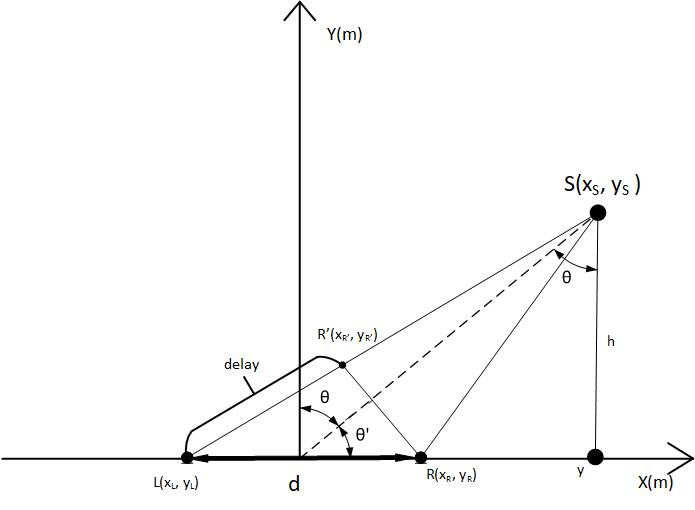
\includegraphics[width=1\textwidth]{Illustrations/mathematicalShit.jpg}
	\caption{Mathematical Interpretation}
	\label{fig:zoomedin2}
\end{figure}

Firstly, the distances SR and SL must be determined. This can be found by employing 
basic trigonometry. This is done by independently finding out the sides of the triangles
SyL  and SyR.

\begin{equation}
	yR = sin(\theta) - \dfrac{d}{2} 
\end{equation}

\begin{equation}
	yL = sin(\theta) + \dfrac{d}{2}
\end{equation}

After the x-coordinates are determined, h is needed in order to calculate the y-coordinates.

\begin{equation}
	h = cos(\theta)
\end{equation}

\newpage
Lastly, the sides SR and SL are determined.

\begin{equation}
	SR = \sqrt{h^2 + yR^2}
\end{equation}

\begin{equation}
	SL = \sqrt{h^2 + yL^2}
\end{equation}

Once the distances are known, the difference in distance between the signals can be found.

\begin{equation}
	delay = SL - SR
\end{equation}

At this moment, the delay is expressed in distance. By knowing the speed of sound, the amount of
time it takes to travel that distance can be found.

\begin{equation}
	delayInTime = \frac{delay}{speed of sound}
\end{equation}

The time, can be converted in amount of samples by multiplying it by the sampling frequency.

\begin{equation}
	delayInSamples = delayInTime * SamplingFrequncy
\end{equation}

\newpage
\section{Idea for filtering}

\begin{figure}[htp]
	\centering
	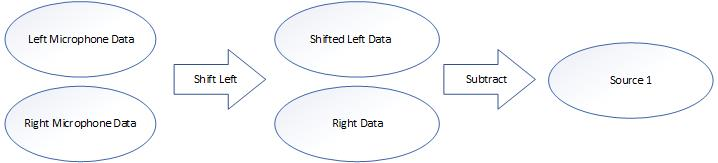
\includegraphics[width=1\textwidth]{Illustrations/IdeaDiagram.jpg}
	\caption{Idea diagram}
	\label{fig:IdeaDiagram}
\end{figure}

Filtering sound, based on the direction that it's coming from could work by taking data, recorded by one of 
the microphones, in this case (figure
\ref{fig:IdeaDiagram}) we chose left microphone data. Then we shift this data by exact amount of samples, 
which would make the source we would like 
to separate recorded by left microphone, exactly aligned with same source, recorded by right microphone.\\
Then by subtracting right microphone data from shifted left, we should get all the other sounds except the 
ones from source we would like to
separate, this is what we will call noise in directional filtering.\\
Separating could be done by taking the original data, putting it to one channel. Then subtracting noise from 
the original data should leave us only
with "clean" sound from the direction, we are interested in.\\
\section{Development}
\todo{MENTION WHERE EACH SUBSECTION COMES IN PLAY}
\subsection{Finding delay in samples}
By setting the angle of what we want to separate our signal at, we can calculate how big shift in samples 
that would account for. We are using this 
delay later, in the directional filtering. Calculations involve using selected angle, gap between 
microphones, sampling frequency of used 
microphones and the 
speed of sound. \\
\todo{DO WE WRITE ABOUT MATH AND EQUATIONS IN MATLAB HERE OR DO WE JUST SKIP IT.}
\subsection{Recording samples}
First, in order to record two microphones in separate tracks directly to computer, we need to give access to 
multiple inputs and outputs,  
independently to computers' sound card. To achieve that audio driver caller ASIO4ALL was used. Using this 
driver, together with recording software, 
which supports multiple input recording, we were able to record different situations with two microphones at 
the same time. \\
\todo{process of setting up for first recordings. Last sentence counters delay paragraph in Filtering section 
(4.3.3)}
Recording with two microphones was set in a quiet room with sound panels on the walls and curtains, all of 
which reduces echo. Using ruler as a guide microphones were set in place and then angles were marked as 
guides to know from which direction sound is coming from. (Figure \ref{fig:recSetup}) 
\begin{figure}[htp]
	\centering
	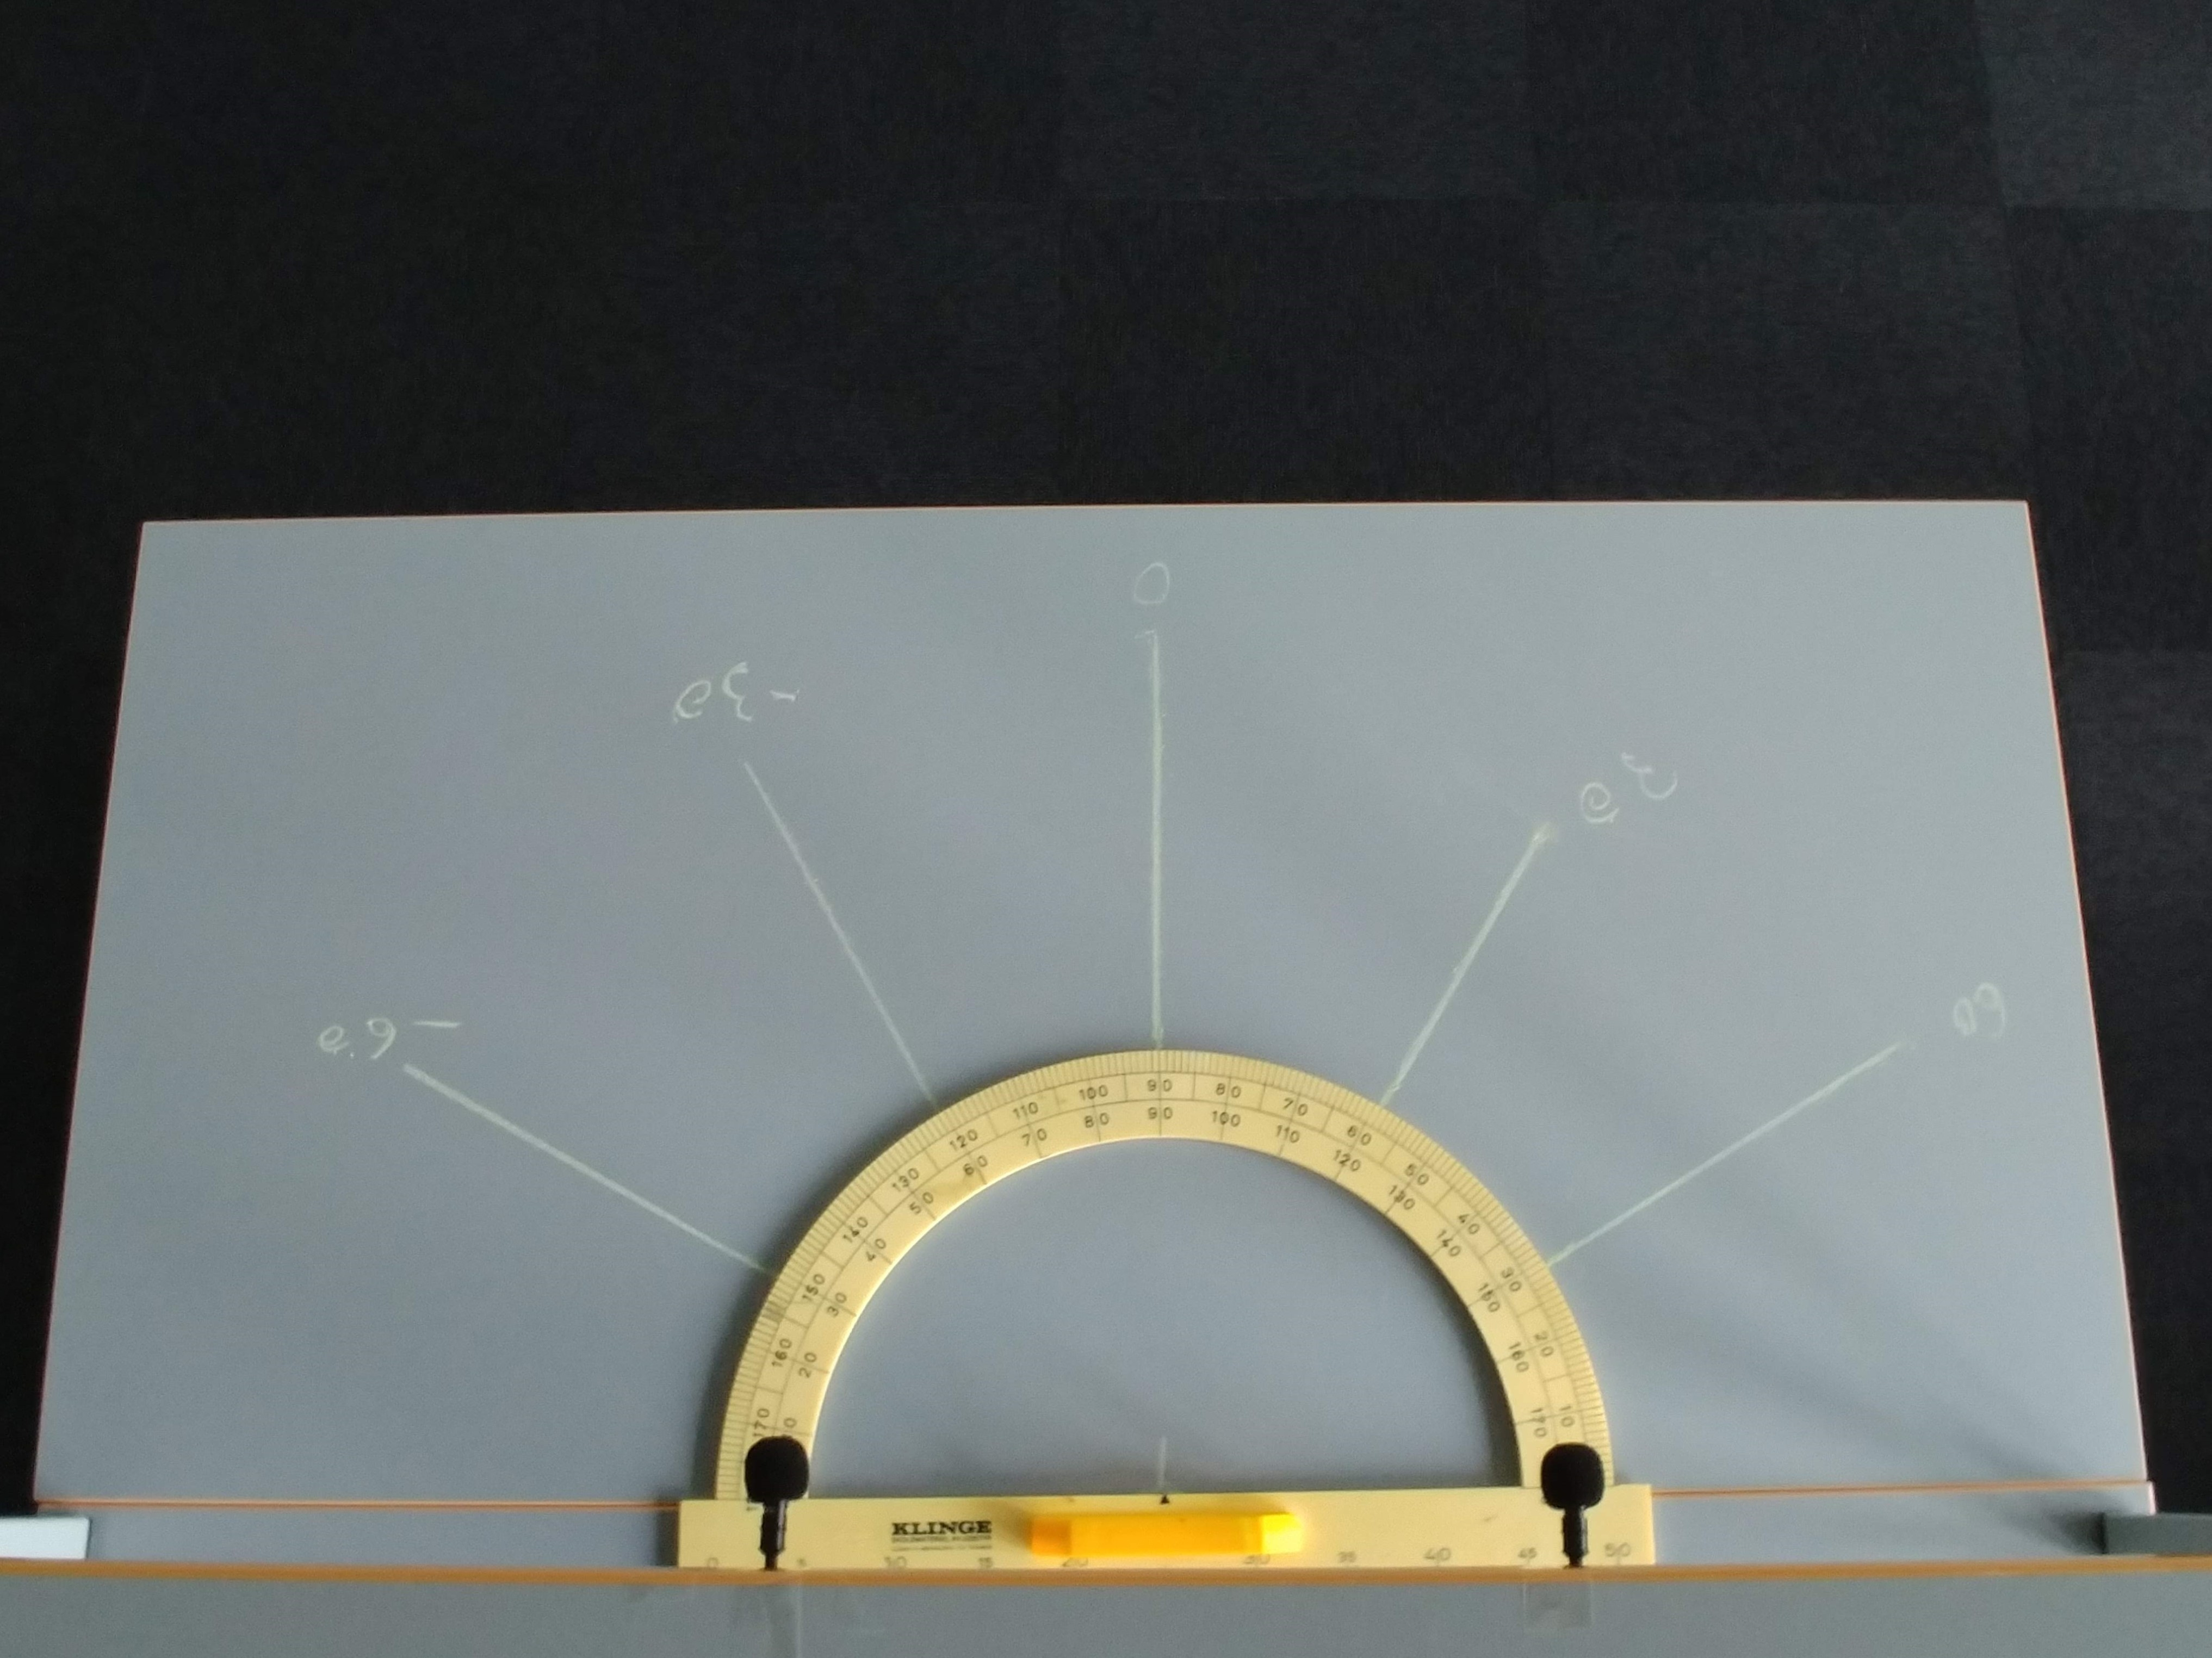
\includegraphics[width=1\textwidth]{Illustrations/JustSetup.jpg}
	\caption{Setup for recording}
	\label{fig:recSetup}
\end{figure}

\subsection{Filtering}
All of the directional filtering is done by applying the logic discussed before to the Matlab script.\\
Prior to shifting signals and filtering, we had to remove any delays, induced by hardware or software. This 
issue was resolved by starting every recording with loud, sharp sound like a clap or a finger snap right in 
the middle of the microphones. Using this sound in the beginning we could match loudest peaks, thus 
eliminating hardware and software induced delay. \\
To see if we can get the samples, which show that logic behind direction of delay is correct, we set up a 
recording with just one person first see figure \ref{fig:RanzvanRecSetup}.\\

\begin{figure}[htp]
	\centering
	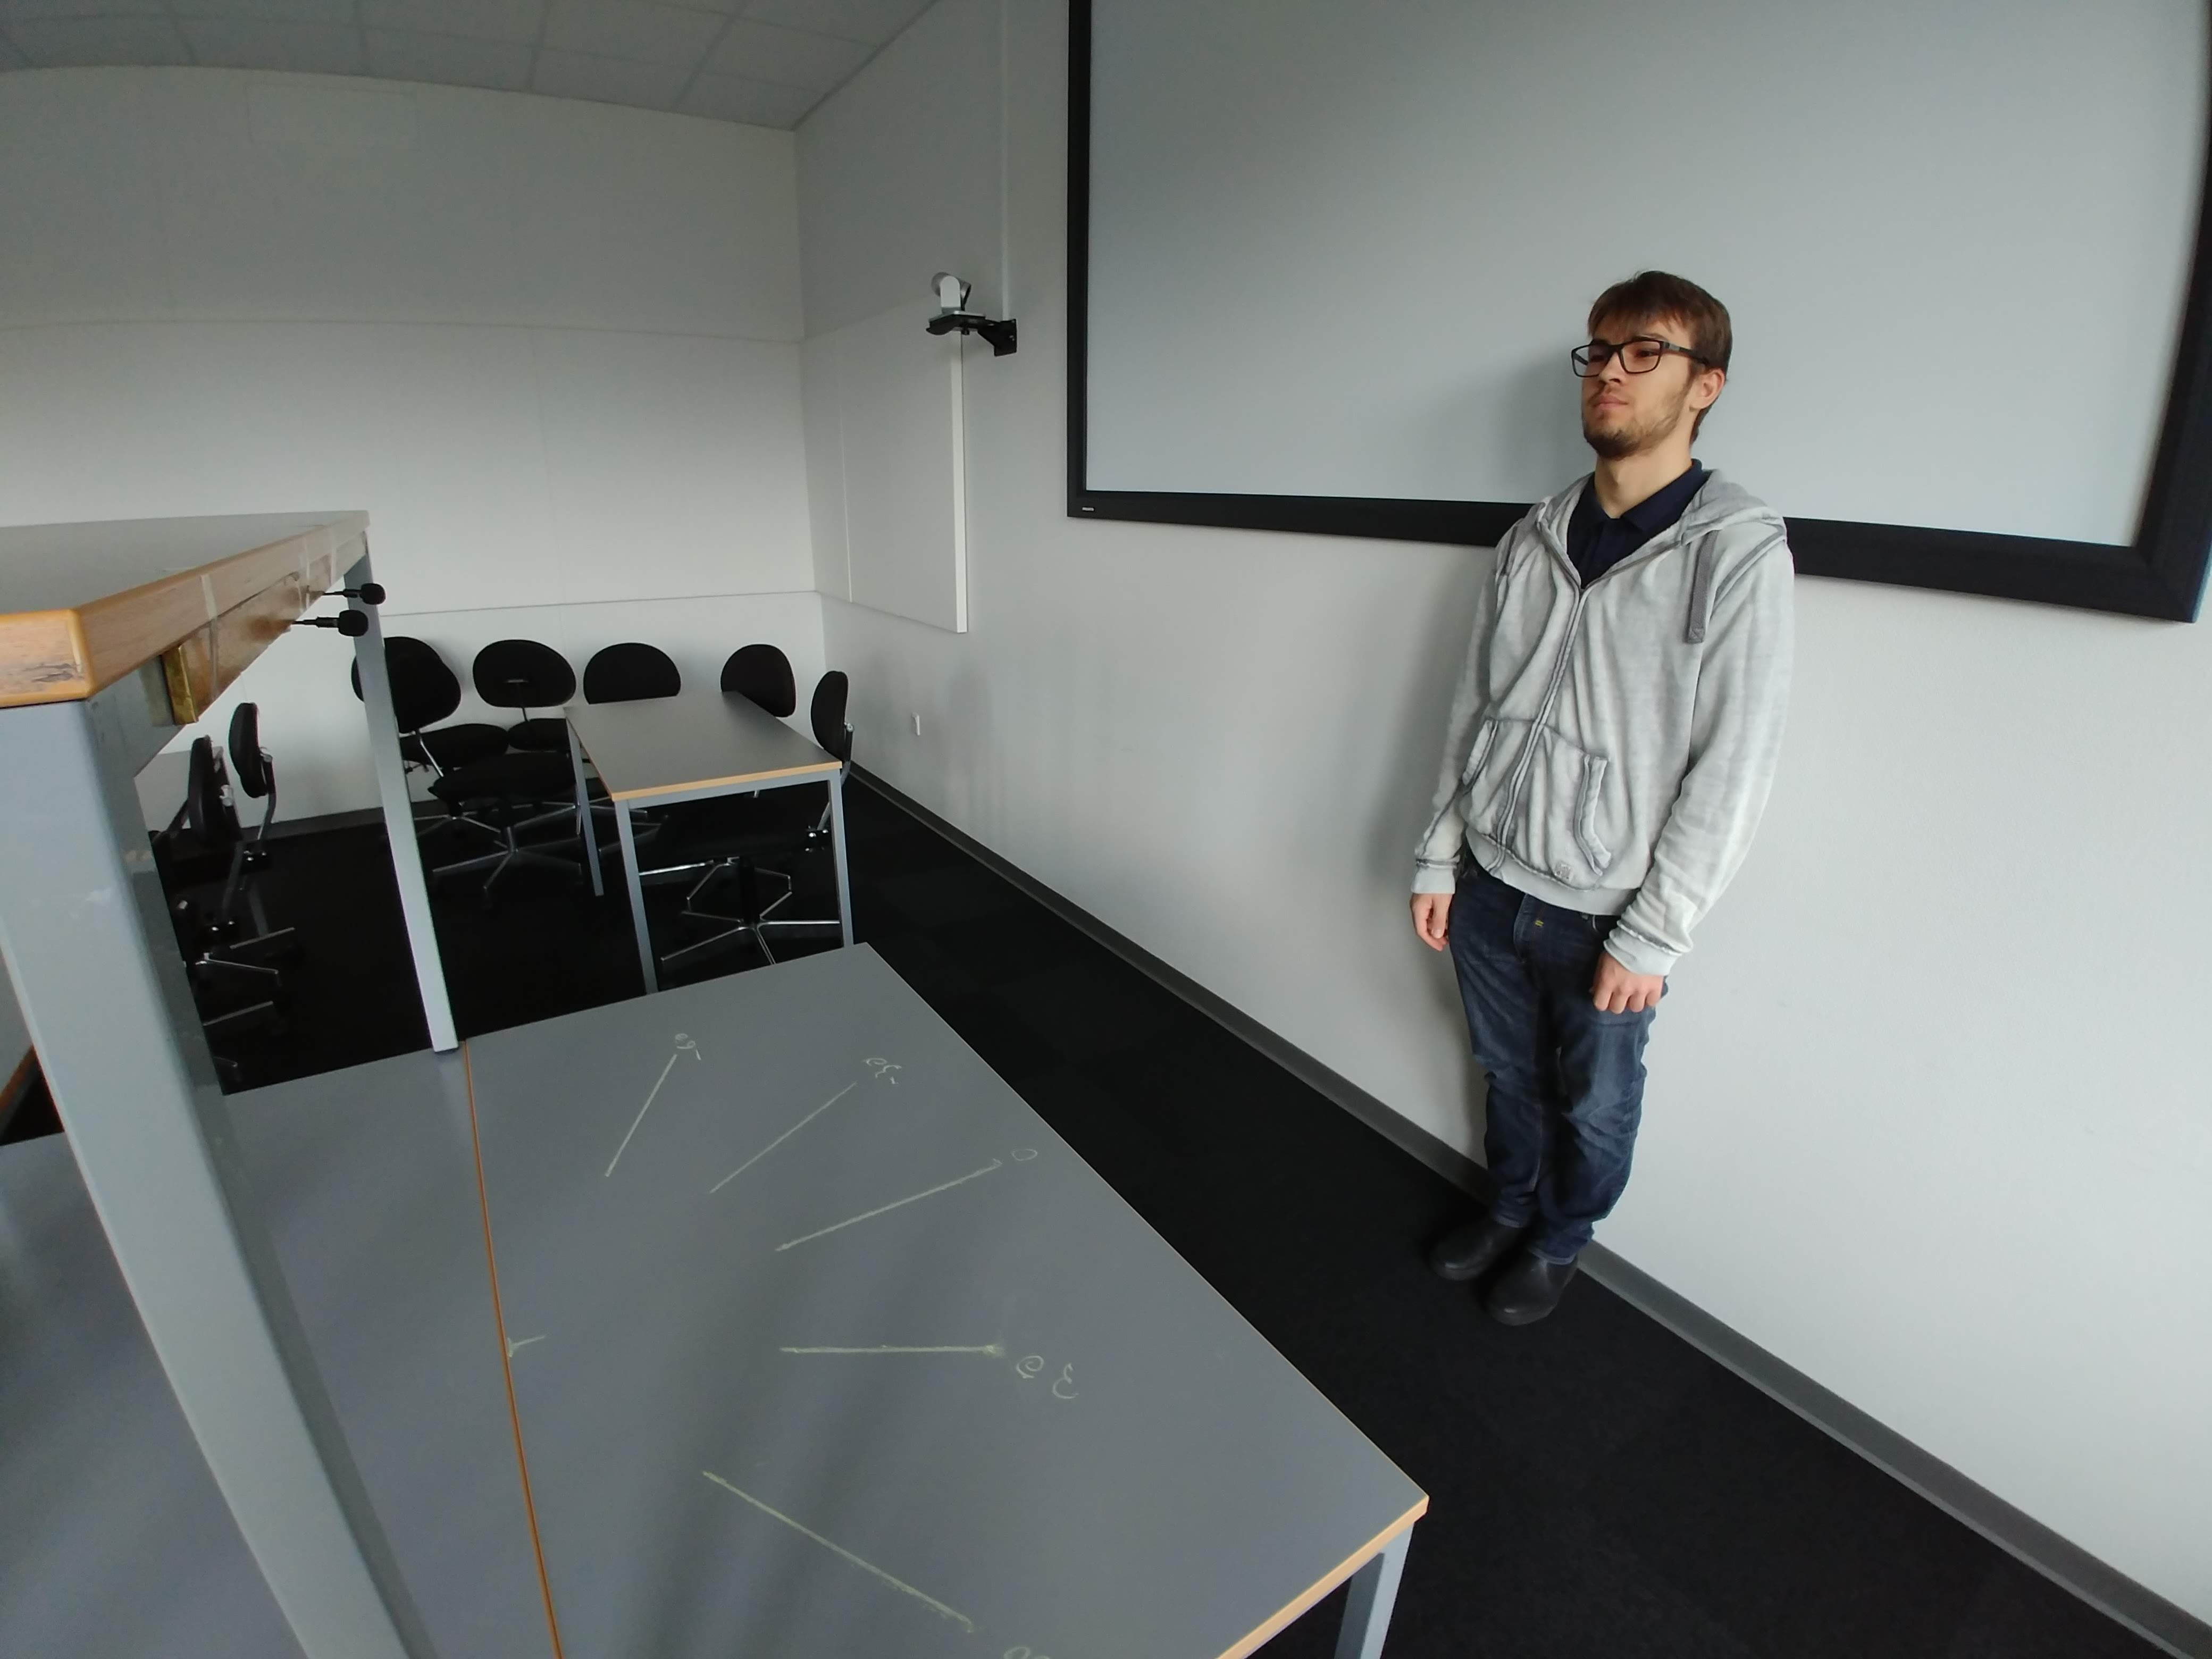
\includegraphics[width=.7\textwidth]{Illustrations/razvanWithSetup.jpg}
	\caption{Setup for recording with a person}
	\label{fig:RanzvanRecSetup}
\end{figure}

Then we looked at collected data:\\
When person spoke from the center, (Figure \ref{fig:C}) shows that recordings match in phase. Green graph is 
data, captured by left microphone and yellow graph is data, captured by right microphone.
\begin{figure}[htp]
  \centering
  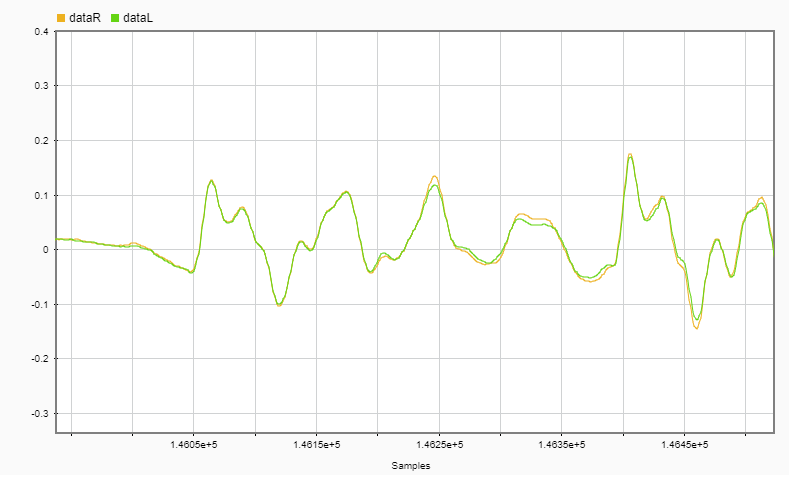
\includegraphics[width=0.75\linewidth]{Illustrations/DataC.png}
  \caption{Data from speaker in the center}
  \label{fig:C}
\end{figure}
\\
\\

When person spoke from the right, right microphone data led left microphone (Figure \ref{fig:R}), here blue graph is left microphone data and orange graph represents right microphone data.\\
\begin{figure}[htp]
  \centering
  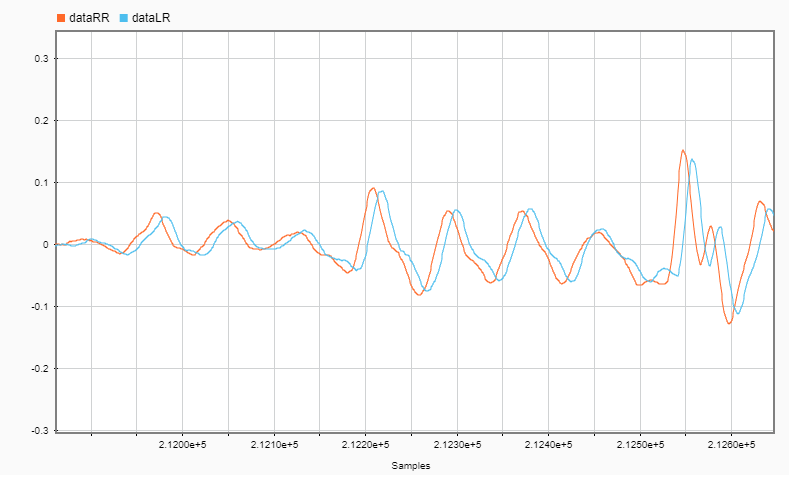
\includegraphics[width=0.75\linewidth]{Illustrations/DataR.png}
  \caption{Data from speaker in the right side}
  \label{fig:R}
\end{figure}

When he spoke from the left, left microphone was leading the right (Figure \ref{fig:L}) pink graph is left microphone data and purple graph shows right microphone data.\\

 
\begin{figure}[htp]
  \centering
  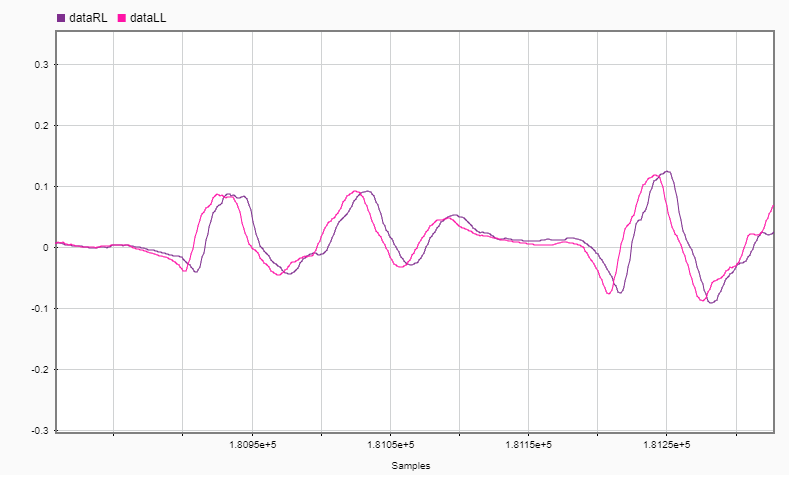
\includegraphics[width=0.75\linewidth]{Illustrations/DataL.png}
  \caption{Data from speaker in the left side}
  \label{fig:L}
\end{figure}

\todo[inline]{"For range -1 to 1 20*log10(x) corresponds to dB" Mention?}
 

All of the directional filtering is done by applying the logic discussed in the Idea for filtering section to 
the Matlab script.\\
First we took data from the recording with only one person, shifted left microphone to match right microphone 
data in phase, then subtracted right microphone data from shifted left microphone data - got "Noise". To 
finish filtering we tried to subtract "Noise" from the Right microphone data.\\
After re-listening the output files from this filtering process (noise file and output file), we couldn't see 
any difference in the output file, compared to the original data. The noise file contained enough data to 
still hear what the person was saying. Our expectation was to hear relative silence in noise file and have a 
bit more isolated output file.
\todo[inline]{"Do we put graphs of noise, output and original data?}
 

\section{Conclusion}